
\documentclass[12pt,a4paper,oneside]{article}
\usepackage[margin=1.2in]{geometry}
\usepackage{appendix}
\usepackage[dvips]{graphicx}
\usepackage{epsfig}
\usepackage{amsmath}
\usepackage{amssymb}
\usepackage{psfrag}
\usepackage[square, comma,sort,numbers]{natbib}
\usepackage{fancyhdr}
\usepackage[nottoc]{tocbibind}
\usepackage{color}
\usepackage{fixltx2e}
\usepackage{pdfpages}
\usepackage{pdflscape}
\usepackage{booktabs}
\usepackage{graphicx}
\usepackage{float}
\usepackage{afterpage}
\usepackage{subcaption}
\usepackage{lscape}
\usepackage{rotating}
\usepackage{enumitem}
\usepackage{array,tabularx}
\usepackage{fancyref}
%\usepackage[dvipsnames]{xcolor}
\usepackage[colorlinks=true,allcolors=blue]{hyperref}%
\usepackage[table,xcdraw]{xcolor}


\newcommand{\quotes}[1]{``#1''}

\newenvironment{conditions*}
  {\par\vspace{\abovedisplayskip}\noindent
   \tabularx{\columnwidth}{>{$}l<{$} @{\ : } >{\raggedright\arraybackslash}X}}
  {\endtabularx\par\vspace{\belowdisplayskip}}



\pagestyle{fancy}
\title{\Huge The Hat Creek Radio Observatory\\
\vspace{0.5cm}
GReX Electromagnetic interference measurements\\
\vspace{0.5cm}
\normalsize \emph{}
\vspace{3.5cm}
\begin{center}

\includegraphics[height=4cm]{Figures/SETI_institute_logo.jpg}
\end{center}
}
\author{ 
\vspace{1cm}
\Large
\textbf{ Alexander Pollak, Wael Farah, Marc Jacquart} \\
SETI Institute \\ 
339 Bernardo Ave, Suite 200 \\
Mountain View, CA 94043 \\ 
Alexander.Pollak.87@gmail.com\\
}
\date{\today}



\begin{document}
\clearpage\maketitle
\thispagestyle{empty}

\newpage

%----------------------------------------------------------------------------------------
%	General
%----------------------------------------------------------------------------------------

This document summarizes the testing of the GReX electronics EM interferences at the Hat Creek Radio Observatory (HCRO) on April 3rd, 2024.

\section{Measurement setup}
\label{sec:Testing}

The GRex unit is place in the screened room and it's Electromagnetic emissions are recorded by a spectrum analyzer connected to an omnidirectional antenna through a signal amplifier. A schematic of the setup is shown in figure \ref{fig:measurement_setup_schematics}, a list of the components used in table \ref{tab:setup_component_list} and a picture inside the screened room in figure \ref{fig:screened_room_setup}. A list of settings for the spectrum analyser is shown in table \ref{tab:spectrum_analyzer_settings}.

\begin{figure}[H]
\centering
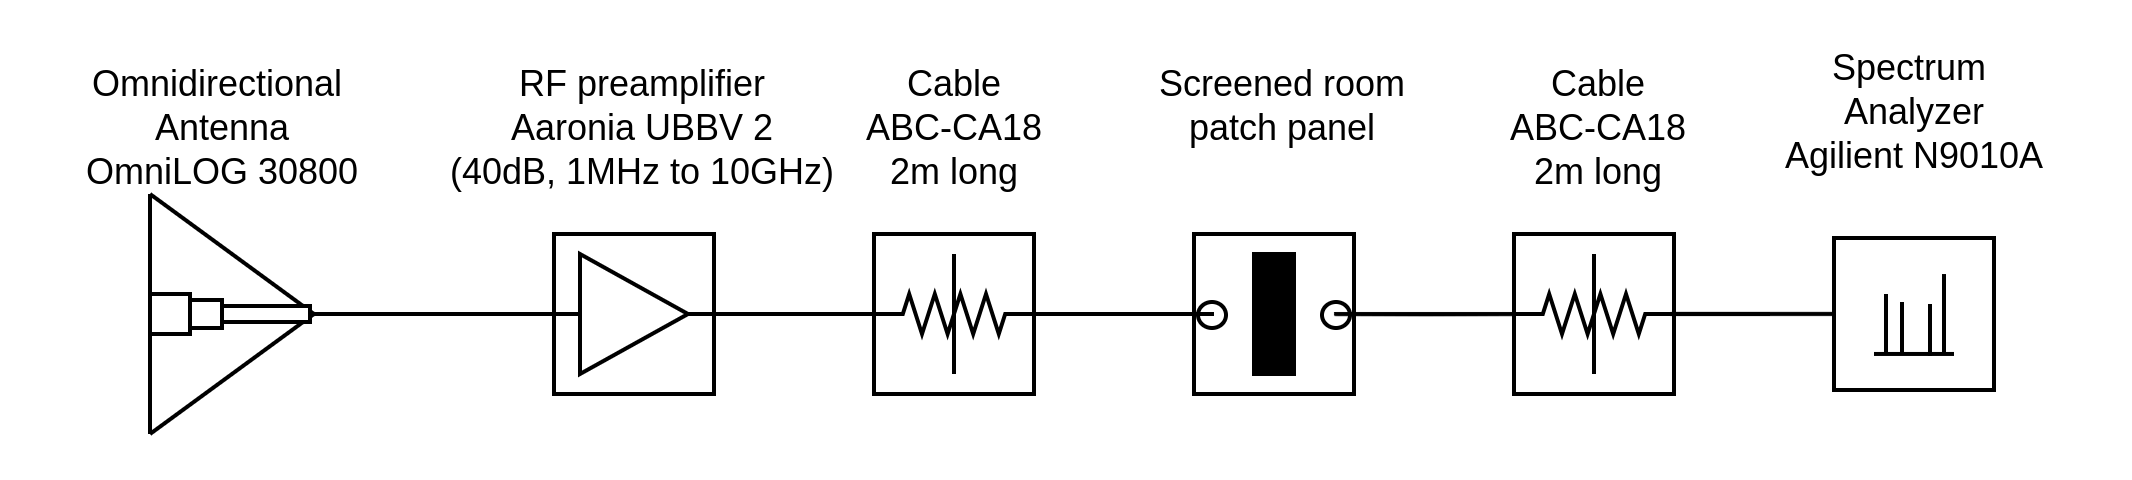
\includegraphics[width=1\linewidth]{Figures/measurement_setup_schematics.png}
\caption{GReX EMI measurement setup schematics.}
\label{fig:measurement_setup_schematics}
\end{figure}


\begin{figure}[H]
\centering
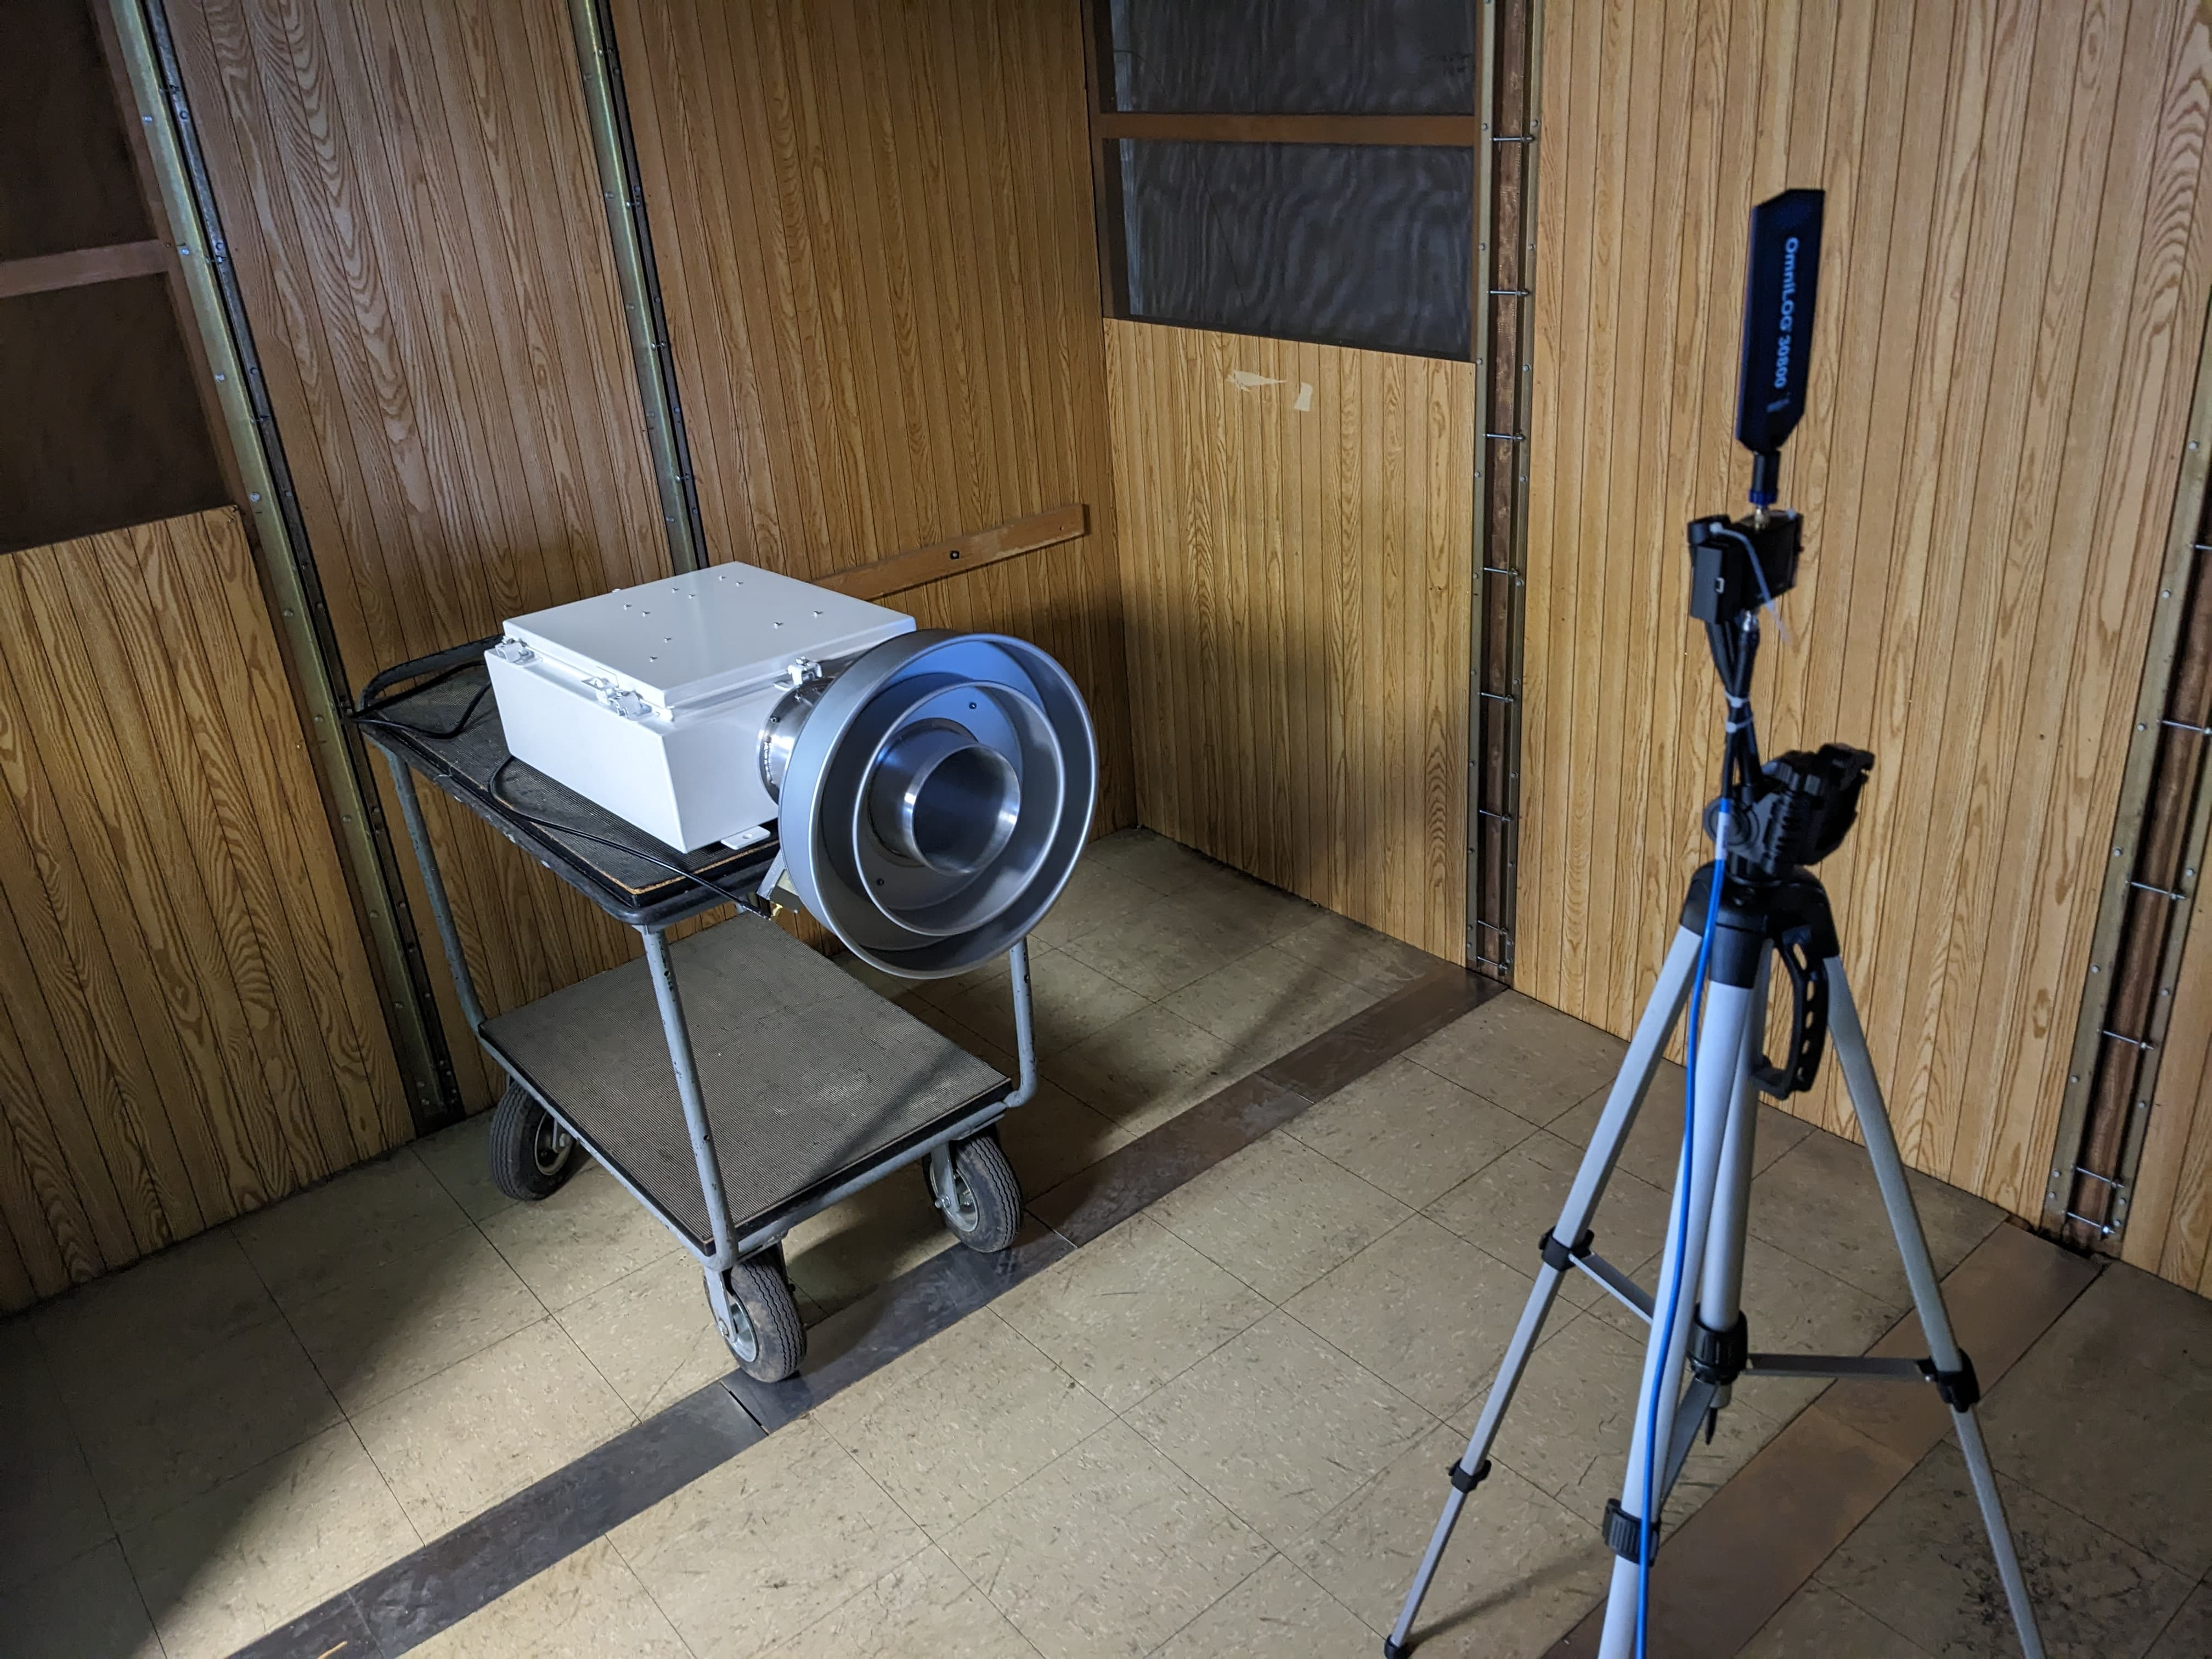
\includegraphics[width=0.8\linewidth]{Figures/screened_room_setup.jpeg}
\caption{Test setup in the HCRO screened room.}
\label{fig:screened_room_setup}
\end{figure}


\begin{table}[]
    \centering
   
    \begin{tabular}{|c|c|}
    \hline
         \cellcolor[gray]{0.85} Description & \cellcolor[gray]{0.85} Designation \\ \hline
         Omnidirectional antenna & OmniLOG 30800\\ \hline
         RF preamplifier & Aaronia UBBV 2\\ \hline
         Female-Female SMA cable 2m & ABC-CA18-SMSM-2.OM\\ \hline
         Female-Female SMA cable 5m & ABC-CA18-SMSM-5.OM\\ \hline
         Spectrum analyzer & Agilent N9010A\\ \hline
    \end{tabular}
    \caption{Measurement setup components list.}
    \label{tab:setup_component_list}
\end{table}

\begin{table}[]
    \centering
   
    \begin{tabular}{|c|c|}
    \hline
         \cellcolor[gray]{0.85} Description & \cellcolor[gray]{0.85} Setting \\ \hline
          Start Frequency & $300\thinspace$MHz \\ \hline
          Stop Frequency & $6\thinspace$GHz \\ \hline
          Number of points & 1001 \\ \hline
          Sweep time & 656.175767597013\\ \hline
          RBW & 100 \\ \hline
          VBW & 1000 \\ \hline
          Attenuation & 0 \\ \hline
          Trace type & Maxhold \\ \hline
          Detector & Peak \\ \hline         
    \end{tabular}
    \caption{Specrum analyzer settings list.}
    \label{tab:spectrum_analyzer_settings}
\end{table}
% ----------------------------------------------------------------
\section{Results}
\label{sec:Results}

The baseline spectrum is shown in figure \ref{fig:baseline_result}. The emission peaks are due to the EMI emitted by the spectrum analyzer itself, eventhough it is set outside the screened room. However, as the comparison spectrum plot shows, this contribution is negligible compared to the GReX measurements recorded. Figure \ref{fig:closed_result} shows the spectrum for the GReX enclosure open is shown in figure \ref{fig:open_result}. The spectrum when the GReX enclosure is closed. Finally, figure \ref{fig:absorber_comparison_spectrum} shows the effect of adding absorbers inside the enclosure. A list of the highest interference peaks, defined as peak $>30\thinspace$dBm abouve their surrounding background, is presented in table X.

\begin{figure}[H]
\centering
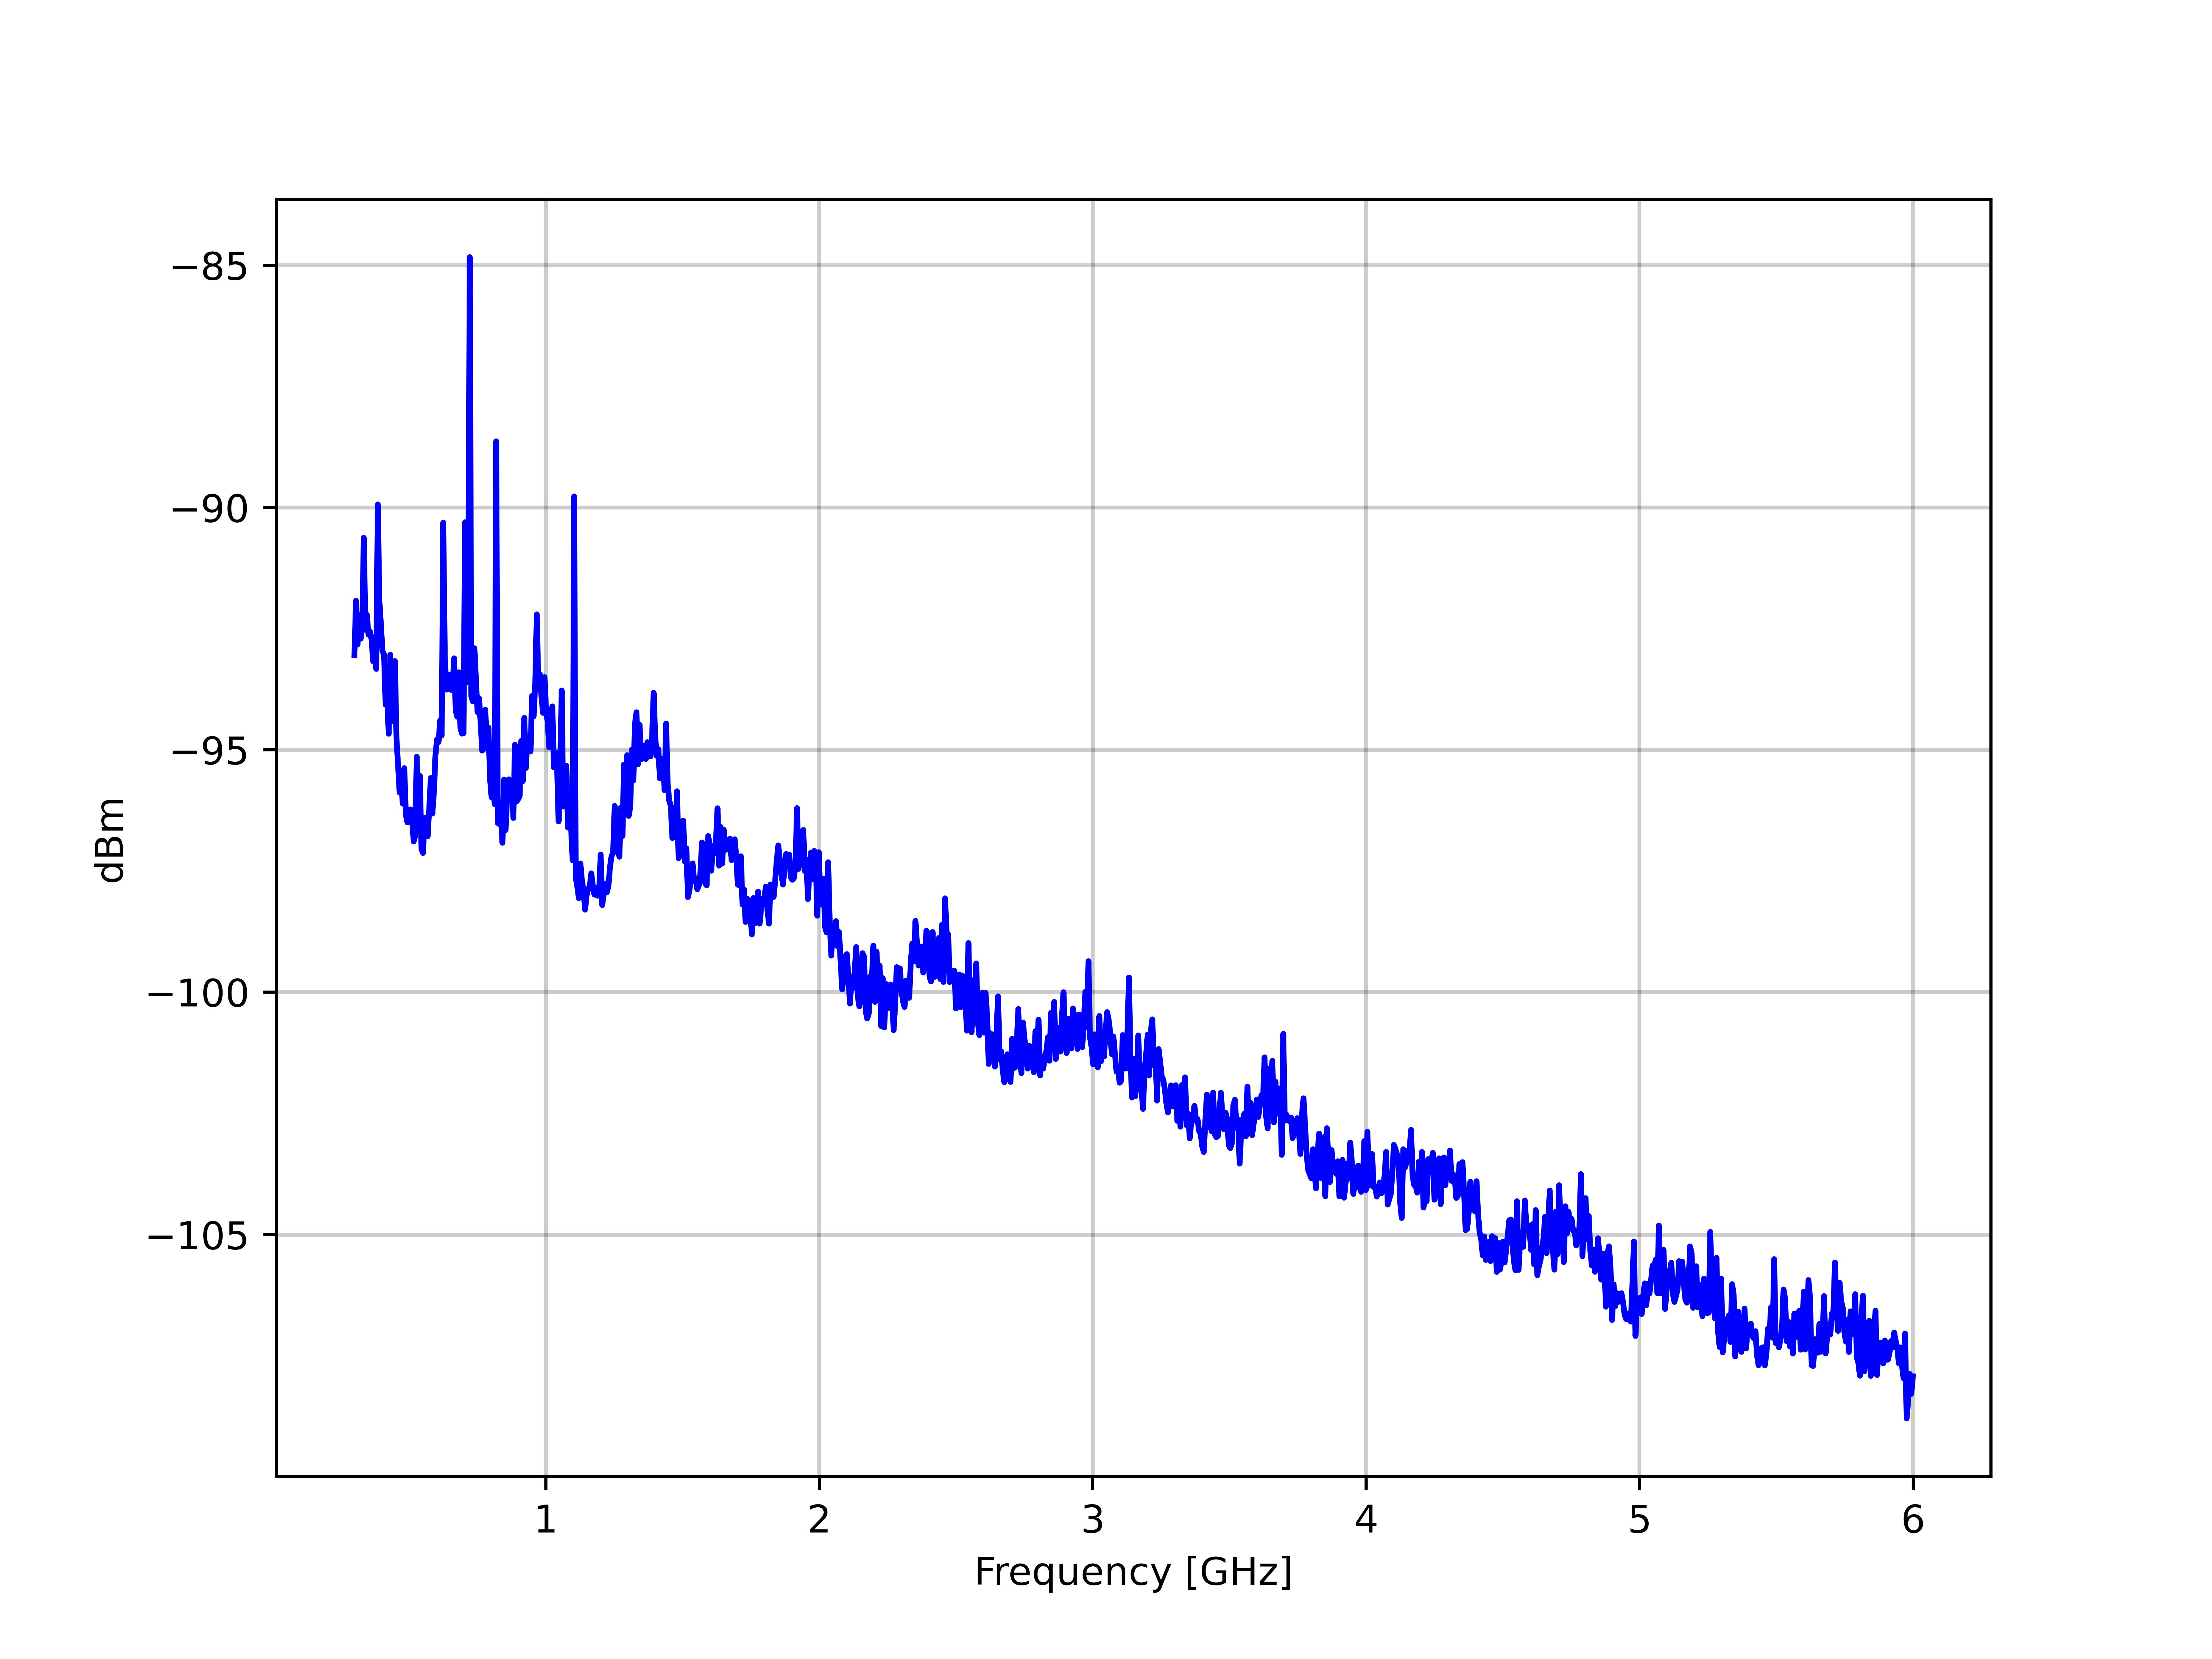
\includegraphics[width=1\linewidth]{Figures/baseline_spectrum.jpg}
\caption{Baseline.}
\label{fig:baseline_result}
\end{figure}

\begin{figure}[H]
\centering
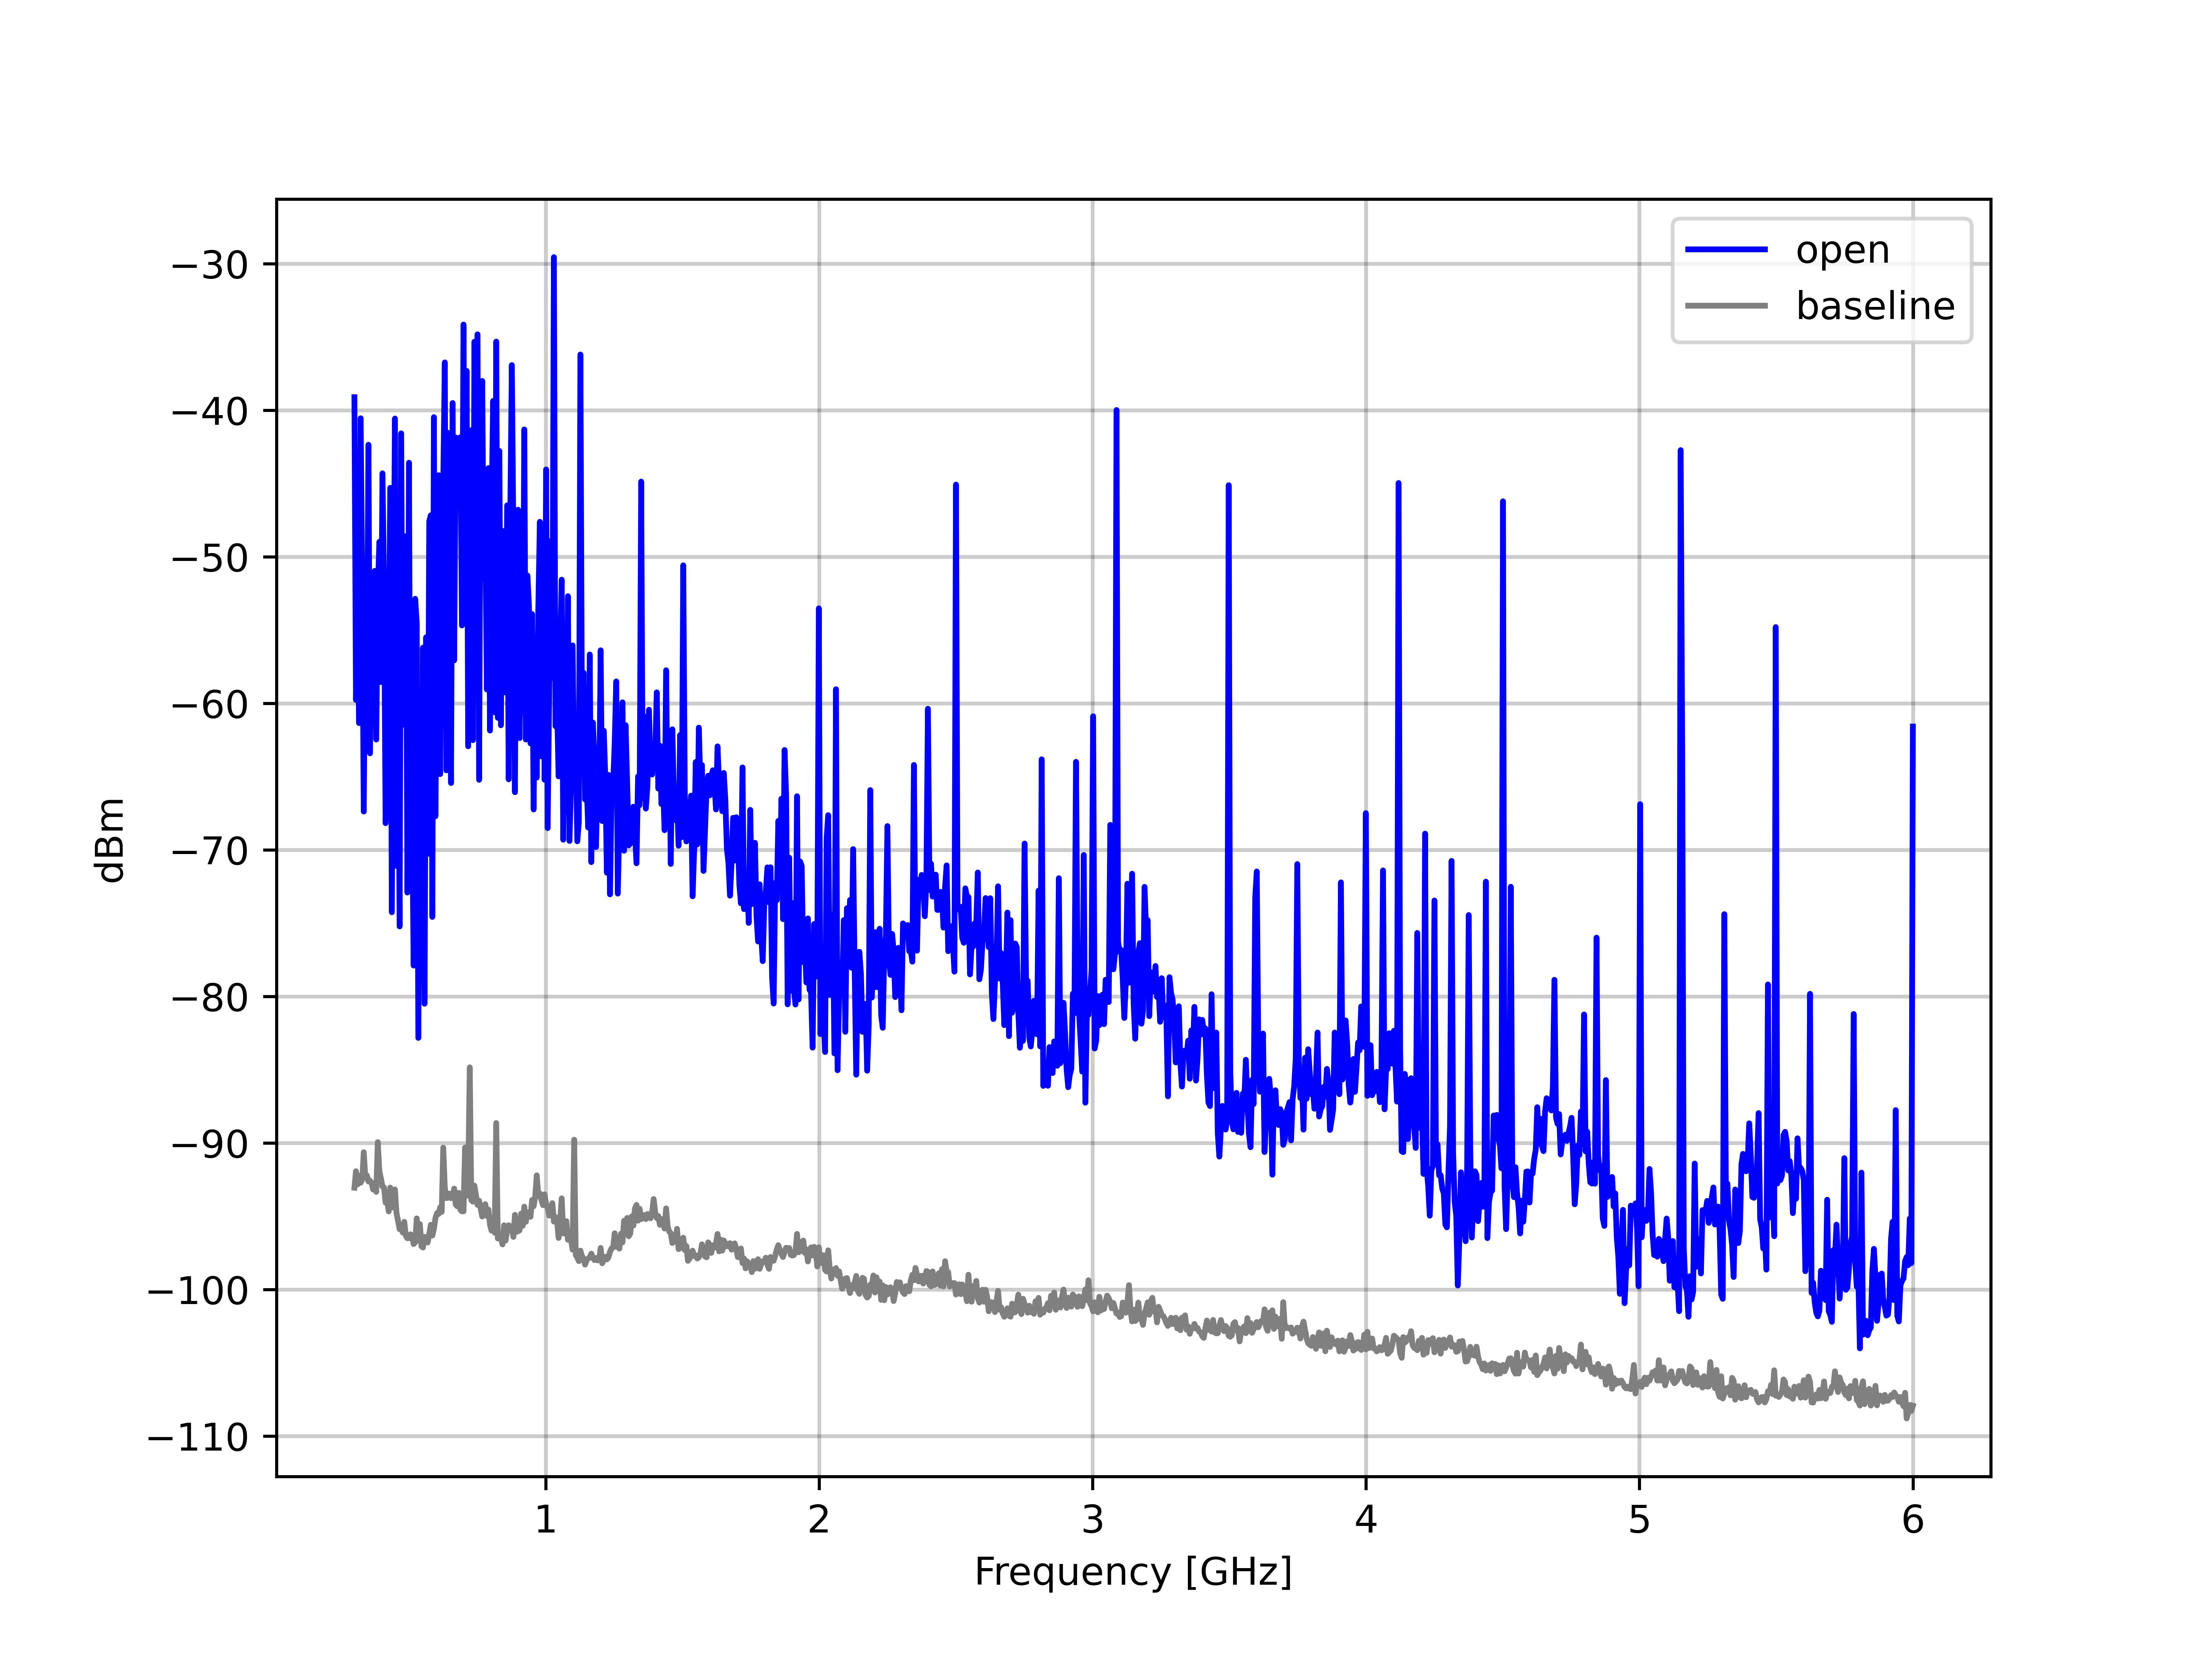
\includegraphics[width=1\linewidth]{Figures/open_comparison_spectrum.jpg}
\caption{GReX enclosure open compared to baseline.}
\label{fig:open_result}
\end{figure}

\begin{figure}[H]
\centering
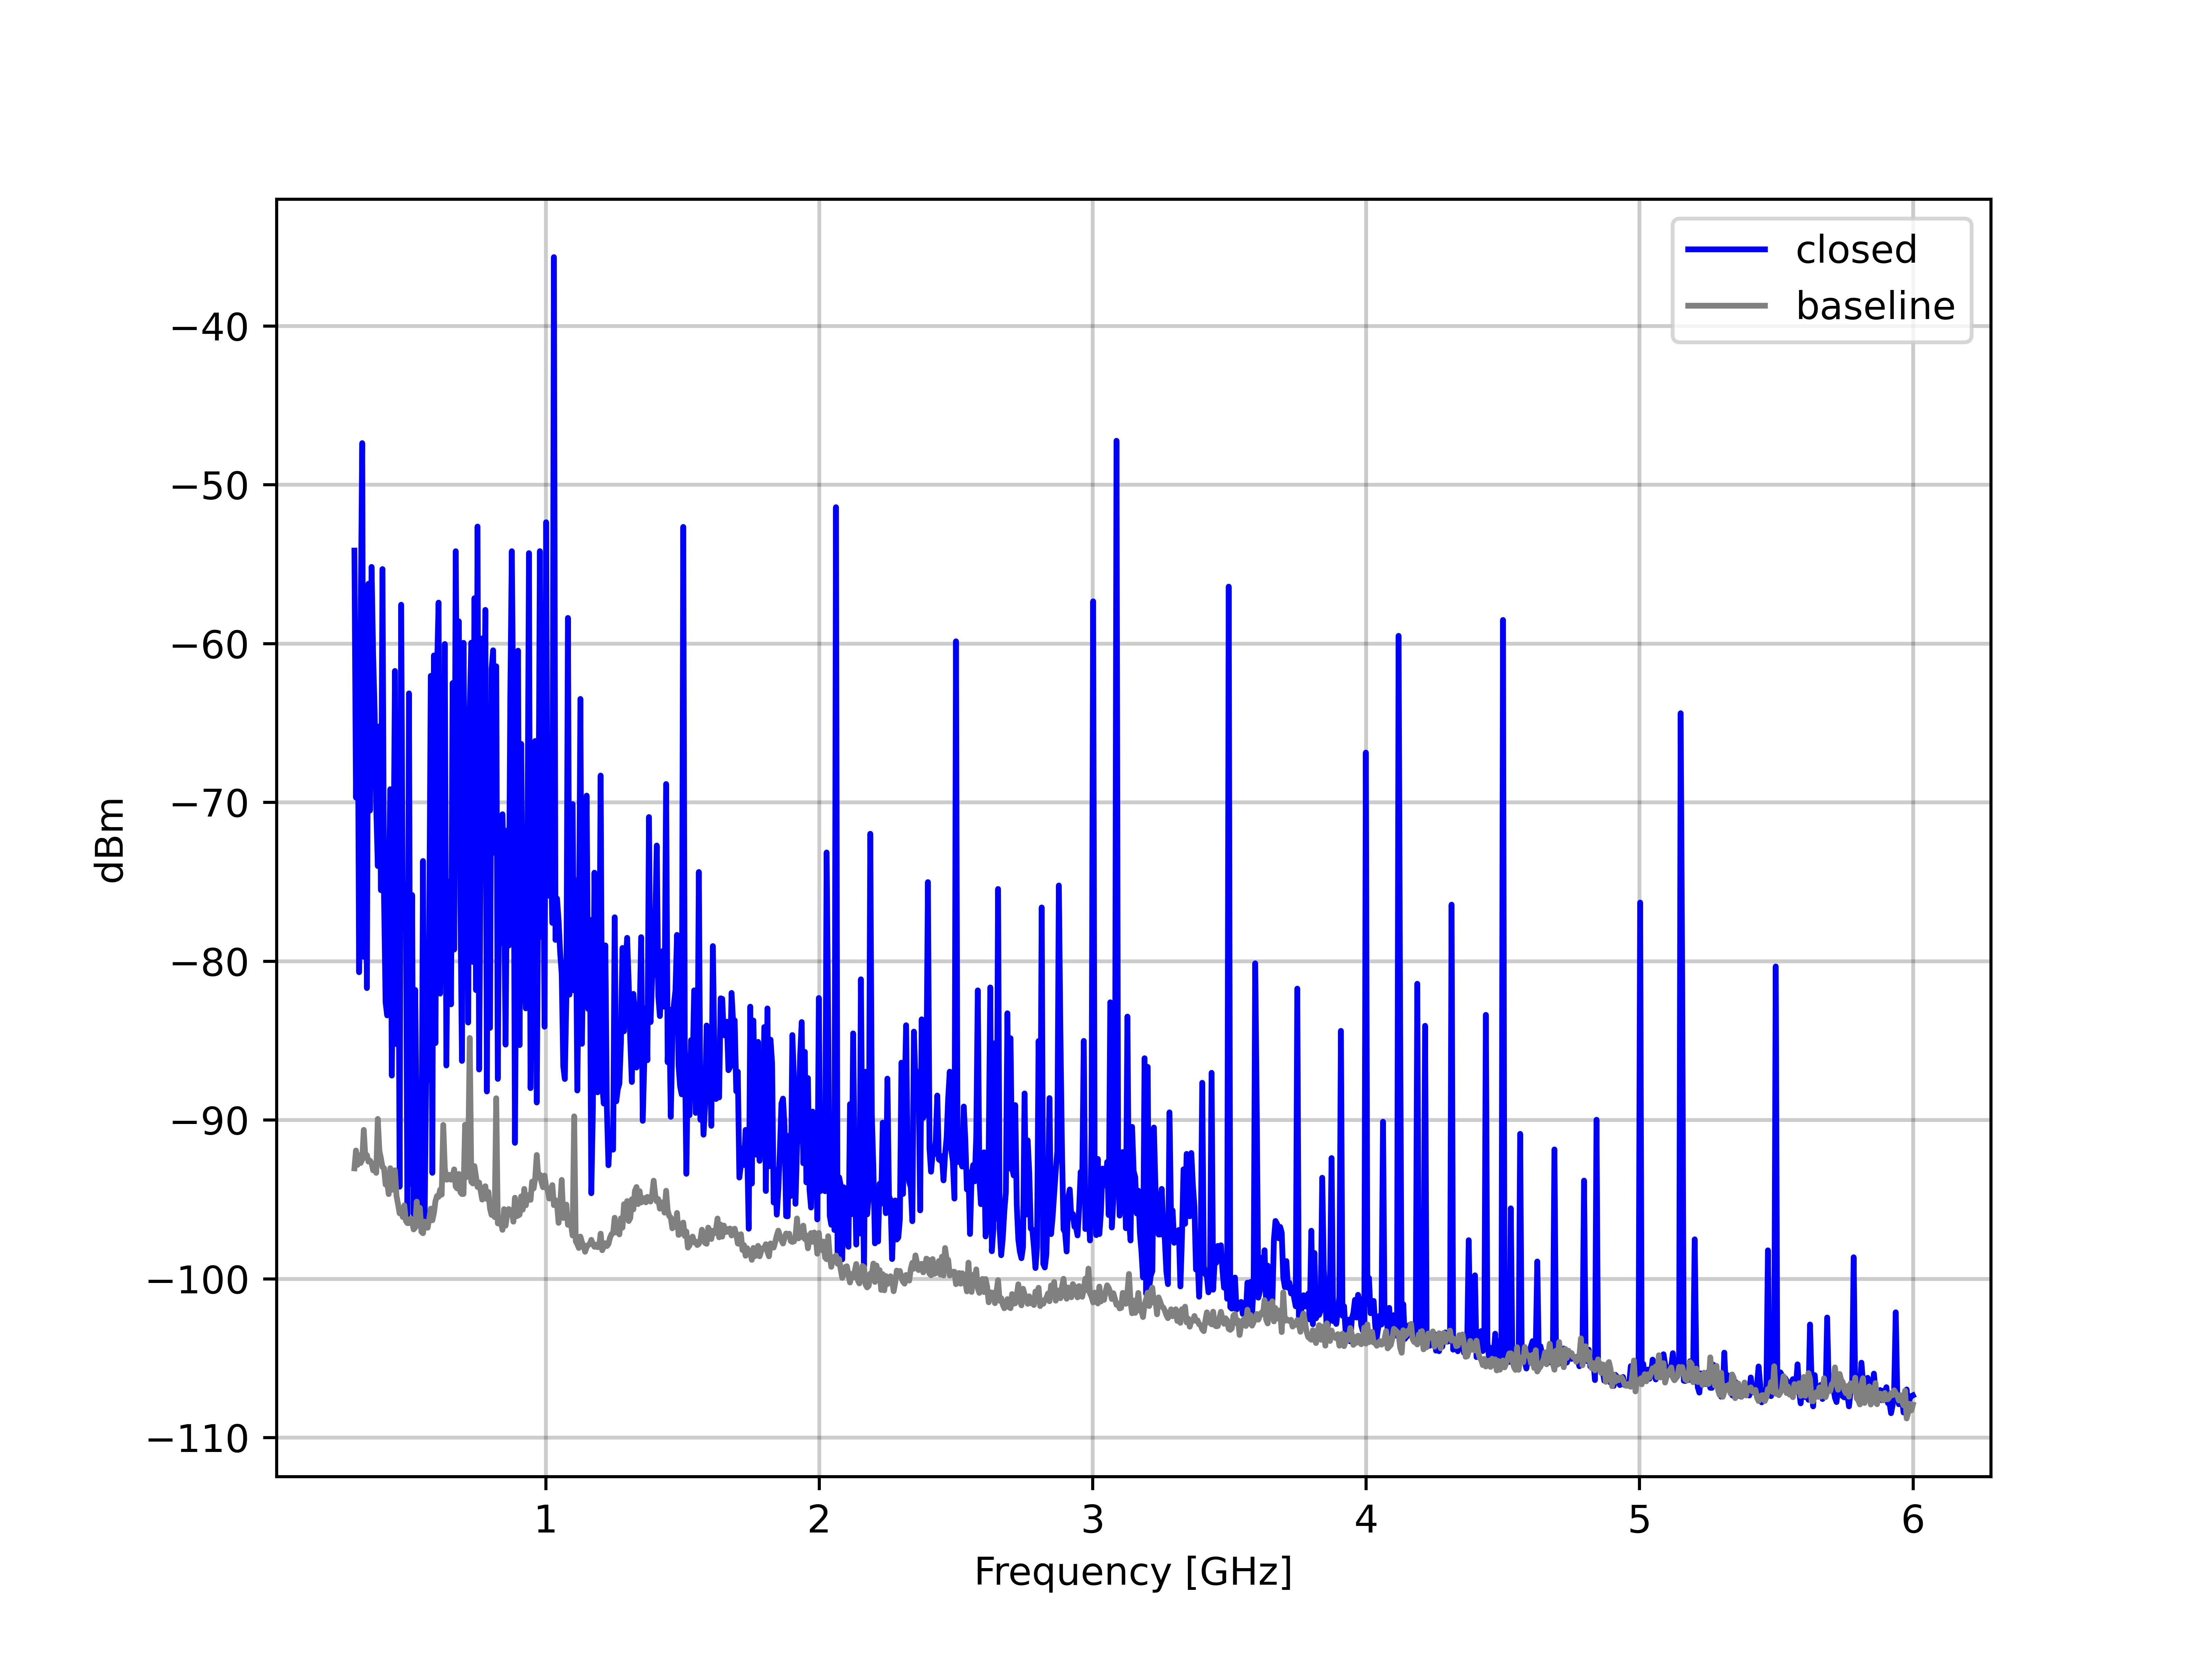
\includegraphics[width=1\linewidth]{Figures/closed_comparison_spectrum.jpg}
\caption{GReX enclosure closed compared to baseline.}
\label{fig:closed_result}
\end{figure}

\begin{figure}[H]
\centering
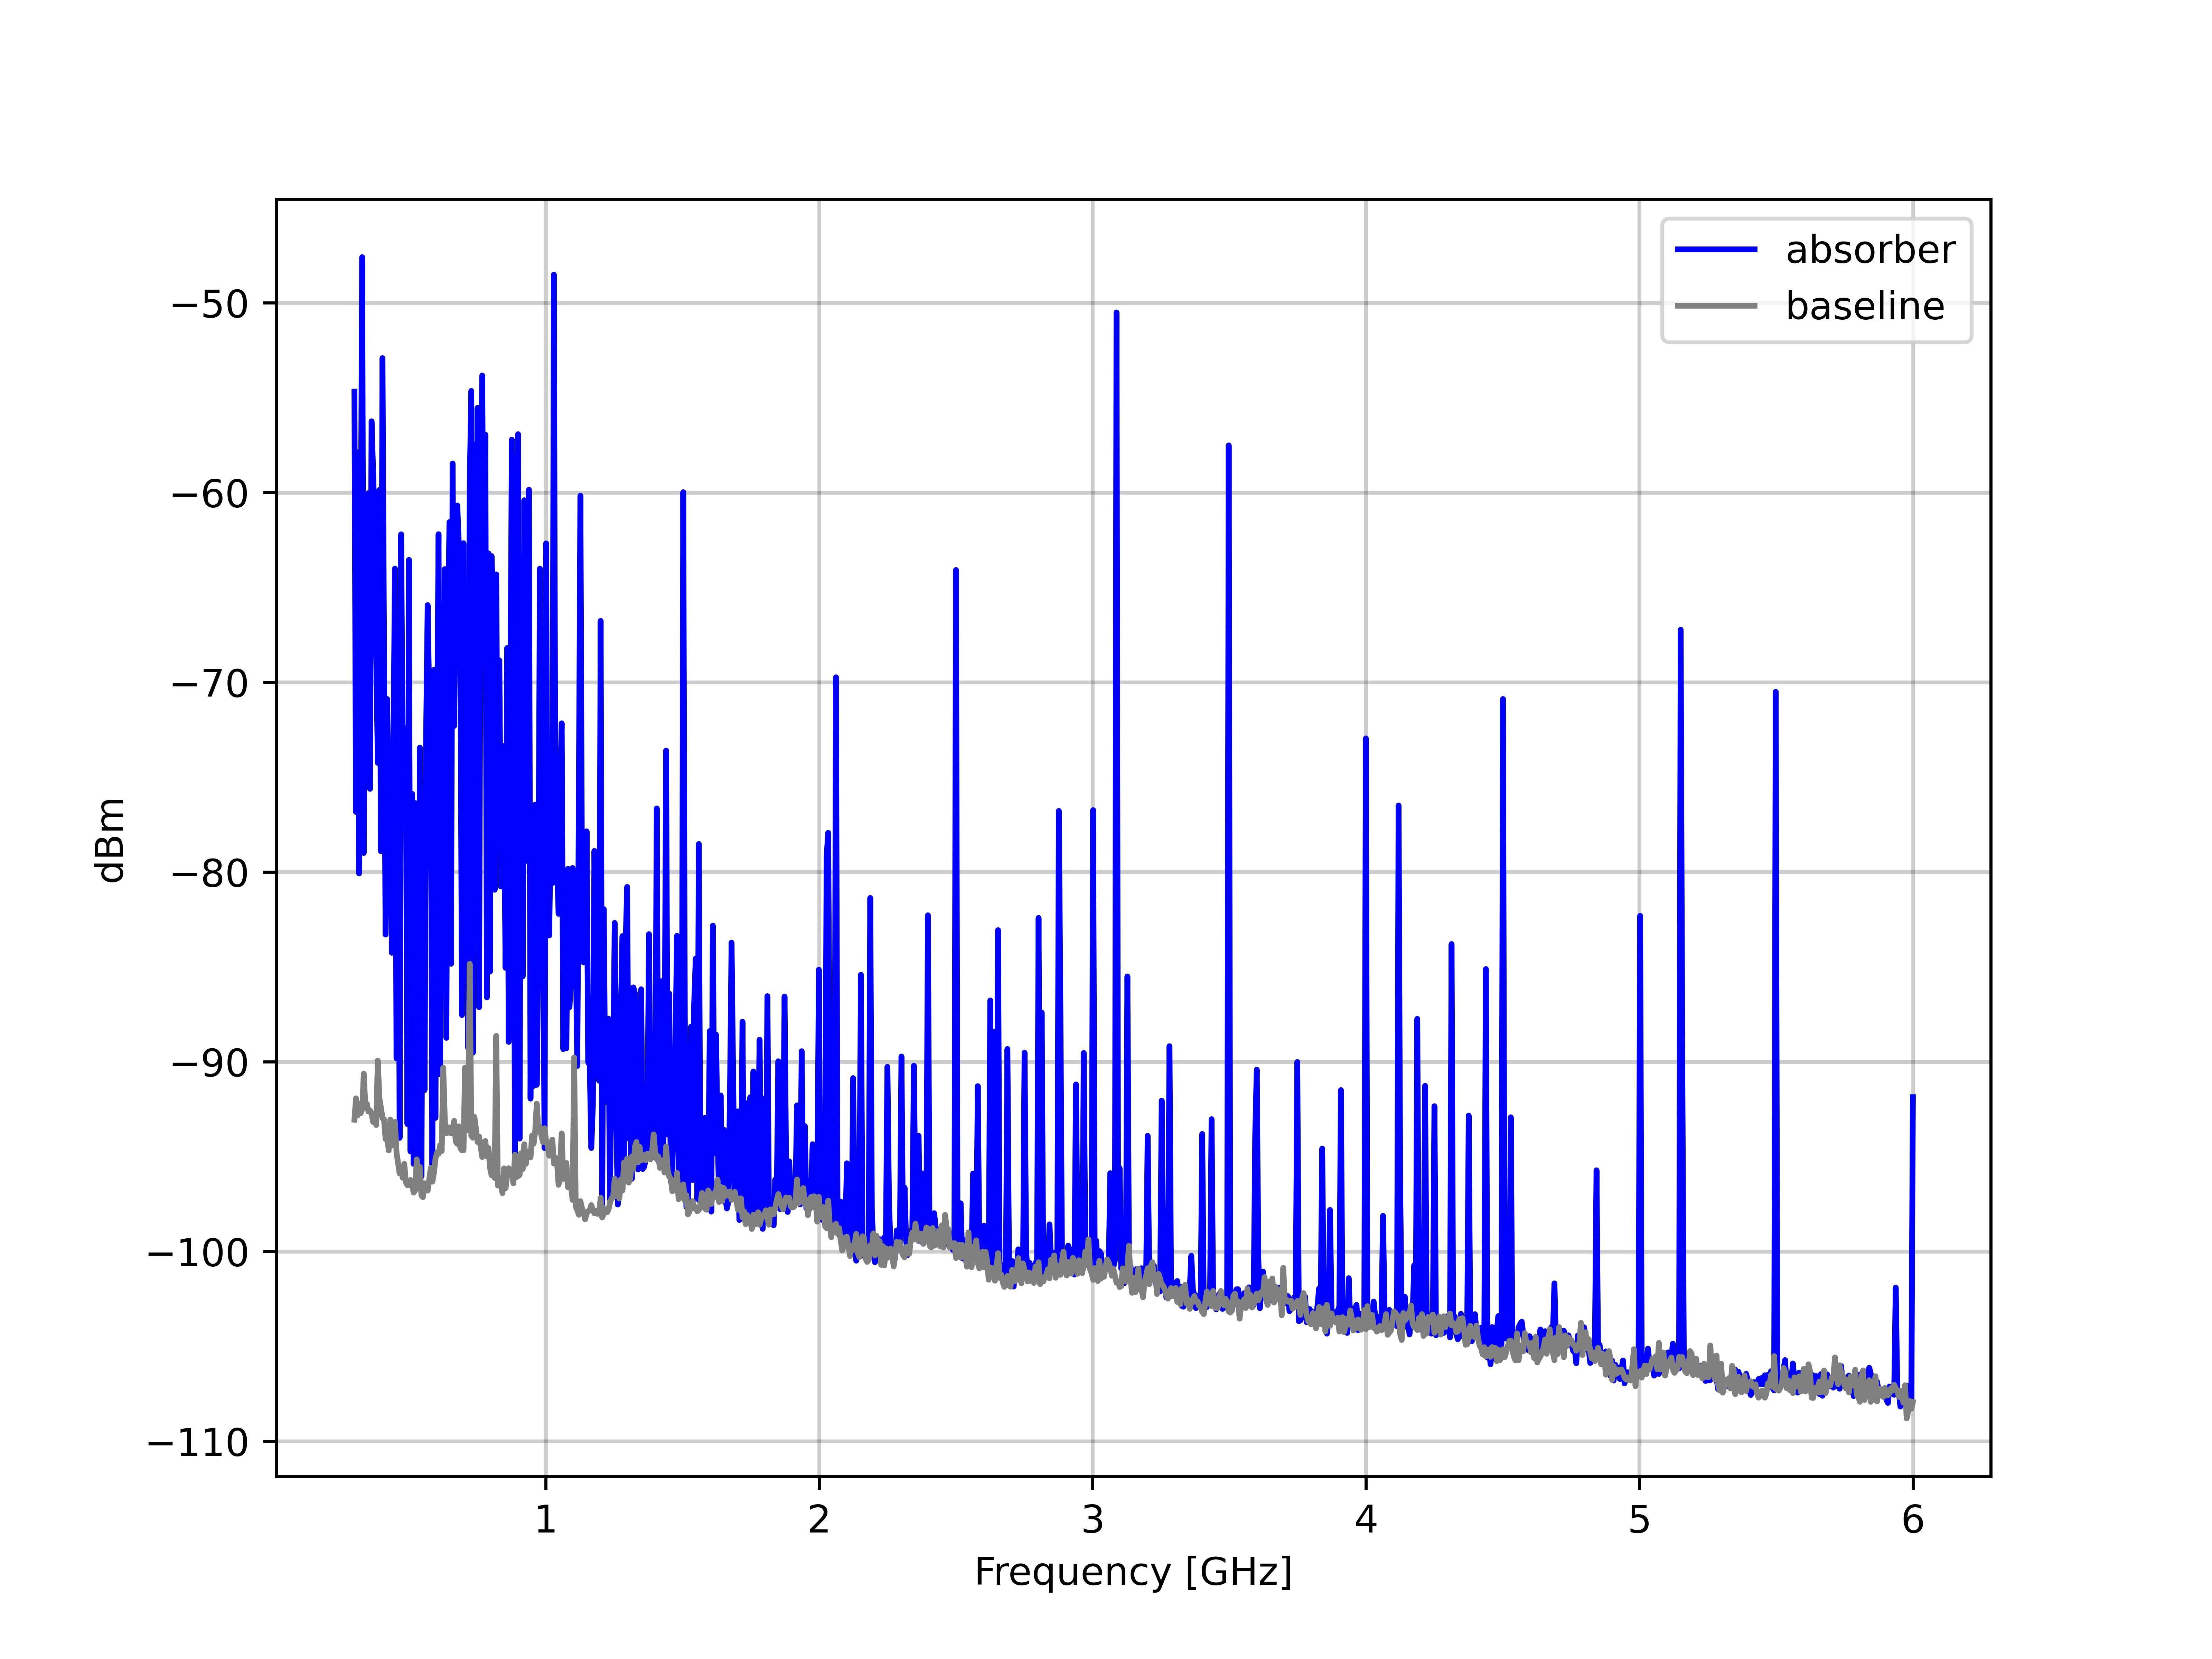
\includegraphics[width=1\linewidth]{Figures/absorber_comparison_spectrum.jpg}
\caption{GReX enclosure closed and compared to baseline.}
\label{fig:absorber_comparison_spectrum}
\end{figure}


\begin{table}[]
    \centering
   
    \begin{tabular}{|c|c|c|}
    \hline
         \cellcolor[gray]{0.85} Measurement & \cellcolor[gray]{0.85} Frequency [GHz] &  \cellcolor[gray]{0.85} Amplitude [dBm]\\ \hline
         closed & 0.4995 & -63.143009 \\ \hline
         closed & 1.0296 & -35.672183 \\ \hline
         closed & 1.5027 & -52.661033 \\ \hline
         closed & 2.0613 & -51.418850 \\ \hline
         closed & 2.5002 & -59.862832 \\ \hline
         closed & 3.0018 & -57.345924 \\ \hline
         closed & 3.0873 & -47.234282 \\ \hline
         closed & 3.4977 & -56.419926 \\ \hline
         closed & 3.9993 & -66.870435 \\ \hline
         closed & 4.5009 & -58.519204 \\ \hline
         & & \\ \hline
         & & \\ \hline
         & & \\ \hline
         & & \\ \hline
         & & \\ \hline
         & & \\ \hline
         & & \\ \hline
         & & \\ \hline
         & & \\ \hline
         & & \\ \hline
    \end{tabular}
    \caption{List of main emission peaks \textbf{verify peaks and condition}.}
    \label{tab:main_emission_peaks}
\end{table}


\end{document}

